%%%%%%%%%%%%%%%%%%%%%%%%%%%%%%%%%%%%%%%%%%%%%%%%%%%%%%%%%%%%%%%%%%%%%%%%%%%%
% AGUJournalTemplate.tex: this template file is for articles formatted with LaTeX
%
% This file includes commands and instructions
% given in the order necessary to produce a final output that will
% satisfy AGU requirements, including customized APA reference formatting.
%
% You may copy this file and give it your
% article name, and enter your text.
%
%
% Step 1: Set the \documentclass
%
%

%% To submit your paper:
\documentclass[draft]{agujournal2019}
\usepackage{url} %this package should fix any errors with URLs in refs.
\usepackage{lineno}
\usepackage[inline]{trackchanges} %for better track changes. finalnew option will compile document with changes incorporated.
\usepackage{soul}
\usepackage{caption}

\linenumbers

% \draftfalse



\journalname{Geophysical Review Letters}


\newcommand{\markred}[1]{\textcolor{red}{#1}}
%\newcommand{\markcyan}[1]{\textcolor{cyan}{#1}}
\newcommand{\markblue}[1]{\textcolor{blue}{#1}}
%\newcommand{\markgreen}[1]{\textcolor{magenta}{#1}}


\begin{document}



\title{Local hydraulic resistance in heterogeneous porous media}


\authors{Quirine Krol\affil{1}, Itzhak Fouxon \affil{1,2}, Pascal Corso \affil{1}, Markus Holzner \affil{1,3,4}}



\affiliation{1}{ETH Zurich, Stefano Franscini-Platz 5, 8093 Zurich, Switzerland}
\affiliation{2}{Department of Computational Science and Engineering, Yonsei University, Seoul 120-749, South Korea}
\affiliation{3}{Swiss Federal Institute for Water Science and Technology EAWAG}
\affiliation{4}{Swiss Federal Institute for Forest, Snow and Landscape Research WSL}



\correspondingauthor{Quirine Krol}{quirine.krol@protonmail.com}



\begin{keypoints}
\item We introduce a new definition for individual pores in heterogeneous porous media based on iso-pressure surfaces.
\item We employ direct numerical simulations to measure the local hydraulic conductivity and revisit the classical model of pore resistance based on Hagen-Poiseuille law. 
\item While Hagen-Poiseuille systematically underestimates low resistances, a new circularity-based model performs significantly better by a reduction of the root-mean-squared-relative error from (on average) $45\%$ to $15\%$.
\end{keypoints}


\begin{abstract}
We examine the validity of the commonly used Hagen-Poiseuille (HP) model of local resistance of porous media. We provide theoretical arguments that highlight possible limitations of this model and formulate a new constitutive model that is based on local pore geometry. We compare the performance of both models on three different three-dimensional artificial porous media obtained by using thresholding on Gaussian random fields. Direct numerical simulations are used to solve the pressure and velocity field of the laminar flow in the pore-spaces of these geometries. We introduce a new definition for pores based on iso-pressure surfaces and topology changes that enables us to measure the local hydraulic resistance. We show that the HP model overestimates the local hydraulic resistance by up to one order of magnitude. Our new model demonstrates that the circularity of iso-pressure surfaces is key to predict the local hydraulic resistances of pores in heterogeneous porous media. This model improves the root-mean-squared-relative error from $59\%$, $48\%$ and $32\%$ for the HP model to $12\%$, $14\%$ and $18\%$ for the three porous media respectively. We anticipate that our approach may find broad application in network models of porous media that are typically build from 3D images with intricate pore geometries.
\end{abstract}

\section*{Plain Language Summary}
[The flow of liquids through porous materials is an everyday problem with many applications ranging from groundwater flow, packed bed reactors, filter devices to blood flow through kidneys. The classical flow modeling approach has been to represent the porous medium as a lattice of circular tubes that represent the pore network and the hydraulic resistance in individual tubes is modeled assuming uniform flow with a parabolic velocity profile, called “Hagen-Poiseuille” law. In this paper we show that this approach has limitations and provide a refined model for local hydraulic resistance based on the pore geometry of complex three-dimensional porous media. In particular, we show that the circularity, i.e., a parameter that quantifies the “roundness” of a surface of equal pressure traversing a pore cross section, is key to predict the local hydraulic resistance.
]


%% ------------------------------------------------------------------------ %%
%
%  TEXT
%
%% ------------------------------------------------------------------------ %%

%%% Suggested section heads:
\section{Introduction}

Porous media flow is important for a wide range of applications in nature and technology, spanning from groundwater remediation and oil recovery to packed bed reactors and particle filters. In these flows, the highly complex and three-dimensional pore geometries give rise to complicated pore velocity fields that form the backbone for transport, mixing and chemical reaction processes. Detailed knowledge of these velocity fields is important for the modelling of effective parameters, most notably the permeability and the prediction of transport in porous media \cite{bear_dynamics_1972,scheidegger_physics_1974}. Despite its importance and extensive research, however, the relation between geometrical features of porous media and the resulting flow is still not fully understood.


Given that detailed knowledge of geometrical features of porous media is often unavailable, the classical flow modeling approach has been to represent the porous medium as a lattice of circular tubes that represent the pore network \cite{scheidegger_physics_1974}. The flow in the tubes is assumed uniform and the velocity profile parabolic. While this is a rather crude approximation of the real geometry and flow behaviors, it has provided useful predictions for flow and transport. Early studies have modelled velocity distributions \cite{haring_statistical_1970}, permeability \cite{fatt_network_1956,katz_quantitative_1986} and particle dispersion \cite{saffman_theory_1959} based on bulk statistics of the medium geometry such as pore size distributions. These early studies have spurred many subsequent works on statistical pore scale models e.g. \citeA{dullien_single_1975,kutsovsky_nmr_1996,maier_simulation_1999,de_anna_prediction_2017} and \citeA{dentz_mechanisms_2018}. The second class of models that hinges on the simplified lattice representation of porous media are the so-called pore network models \cite{thompson_modeling_1997}. For both classes of models, the simplified modelling of local hydraulic resistance of individual pores based on Hagen-Poiseuille is a central element.


Many authors tried to relate the statistics of pore velocity to statistics of pore geometry represented by e.g. the local pore radius and the connectivity between pores. For example, one of the simplest models is the so-called \emph{capillary bundle} model, in which the porous medium is conceptualized as a parallel arrangement of capillaries with given pore sizes \cite{scheidegger_physics_1974}. Extensions of this model include parallel arrangements of wavy tubes \cite{le_borgne_effective_2011}. These simple models are not appropriate for complex porous media, for which the network aspect is important. That is, in general, the connectivity between pores cannot be neglected and the concept of the linear pore breaks down \cite{dentz_mechanisms_2018}. An ad-hoc model that conceptualizes flow in porous media as a system of serial and parallel pore arrangements can be found in \citeA{holzner_intermittent_2015}, and the resulting dispersion of tracers was predicted by \citeA{fouxon_solvable_2016}. \citeA{siena_relationship_2014} and \citeA{hyman_heterogeneities_2012} statistically related velocity distributions to pore size distributions of statistically generated 3D porous media. Based on direct numerical simulations in 2D porous media composed of disks, \citeA{de_anna_prediction_2017} showed that the low velocity tail of the pore velocity distribution is governed by local pore size. This is a notable result as it suggests that the slow flow velocities are not strongly dependent on the connectivity between pores. \citeA{alim_local_2017} showed that pore velocity distributions are governed by local correlations of pore sizes that organize flux ratios at pore junctions, while pore size itself was a poor predictor of flux ratios. They simplified two-dimensional porous medium flow by a network of tubes with varying diameter and the flow within each tube was calculated by solving for Kirchoff’s circuit law for two-dimensional Poiseuille flow within the tubes of rectangular cross section. Even though using tubes with varying diameter is a refinement compared to simpler models with tubes of constant diameter, the simplification with respect to real geometries is still strong. Despite this, a comparison of simulation results with the experimentally obtained velocity distribution in a two-dimensional micromodel composed of pillars showed reasonable agreement \cite{alim_local_2017}. As mentioned, the statistical models in these works are based on the concept that local velocity profiles are parabolic. Some recent papers provided qualitative examples comparing pore velocity profiles to a parabola that suggest the assumption may be reasonable \cite{de_anna_prediction_2017,dentz_mechanisms_2018} and some evidence is provided by the comparison between simulations and experiments by \citeA{alim_local_2017}. However, a rigorous assessment of local hydraulic resistance in three-dimensional pore geometries is still missing in the literature. 


With the advent of experimental techniques like micro-computed tomography there is now access to impressive details of three dimensional porous media architectures. Even though today's computing facilities make it possible to solve flow and transport with unprecedented accuracy in these complex geometries using direct numerical simulations, this approach is only feasible in small domains. Simple models that reduce the full complexity of real porous media are still needed. A lattice representation is the standard approach in so-called pore network models in which a Kirchhoff-type system of equations is solved to model single or multiphase porous medium flows \cite{thompson_modeling_1997} especially in absence of a detailed microstructure. The lattice is usually constructed based on data from experimental pore scale characterization measurements, e.g. imaging or mercury intrusion porosimetry. These pore network models are a valuable tool for understanding meso-scale phenomena, linking single pore processes and continuum porous media used in engineering \cite{xiong_review_2016}. Besides a sound network construction approach that mimics the real media, another critical aspect for the accuracy of modeling is the representation of local hydraulic resistance in the pores. 


In this paper we start with a theoretical background where we define local pores based on consecutive iso-pressure surfaces, followed by a new model for the local hydraulic conductivity. In the methods section we describe our numerical experiment consisting of direct numerical simulations (DNS) from which we obtain local velocity and pressure data in heterogeneous porous media. Based on a post-processing of the DNS data we can extract the local hydraulic conductivity of a local pore. In the results we compare the measured hydraulic resistances to the Hagen-Poiseuille model and to the newly formulated model based a local shape parameter circularity. In the discussion we treat the limitations and extrapolations of the newly proposed model. In the final chapter we provide our conclusions.



\section{Theoretical Background}

For low Reynolds numbers and incompressible flow, the local flow in a porous media is described by the Stokes equations,
\begin{equation}
	\mathbf{\nabla} p =  \mu\mathbf{\nabla}^2 \mathbf{u}\,,~~~\mathbf{\nabla}\cdot\mathbf{u}=0\label{eq:stokes_local}
	\end{equation}
with pressure $p$ and velocity $\mathbf{u}$ and dynamic viscosity $\mu$. For an arbitrary volume $\mathcal{V}$ in a porous media, enclosed by surface $\partial \mathcal{V}$ given by two iso-pressure surfaces $\mathcal{S}_{p_1}$ and $\mathcal{S}_{p_2}$ and solid-liquid surface boundary $\Gamma$, we can write down the integral form of the Stokes equations using the divergence theorem. 
\begin{equation}
\int_{\mathcal{V}} \left(\mathbf{u}\cdot\mathbf{\nabla} p-\mu \mathbf{u}\cdot\mathbf{\nabla}^2 \mathbf{u}\right) dV 
= \int_{\partial \mathcal{V}}  p\,\mathbf{u}\cdot\mathbf{n}\,dS-\mu \int_{\partial \mathcal{V}} \mathbf{u}\cdot (\mathbf{\nabla}\otimes \mathbf{u})\mathbf{n}\,dS+\mu \int_{\mathcal{V}} (\mathbf{\nabla}\otimes\mathbf{u})^2 dV=0, \label{eq:stokes_dissipation}
\end{equation}
with $\mathbf{n}$ the normal vector pointing outwards of surface $\partial V$, and $\otimes$ the dyadic product. Given that at the porous media boundary domain $\Gamma$ we have a no-slip condition $\mathbf{u}=0$ we can write 
\begin{equation}
	Q \Delta p = -\mu\int_{S_{p_1}+S_{p_2}} \mathbf{u}\cdot (\mathbf{\nabla}\otimes \mathbf{u})\mathbf{n}\,dS +\mu \int_{\mathcal{V}} (\mathbf{\nabla}\otimes \mathbf{u})^2 dV, \label{eq:pressuredrop}
\end{equation}
with the total flux through any cross section defined by 
\begin{equation}
	Q=\int \mathbf{u}\cdot\mathbf{n}\, dS.
\end{equation}
\begin{figure}[t!]
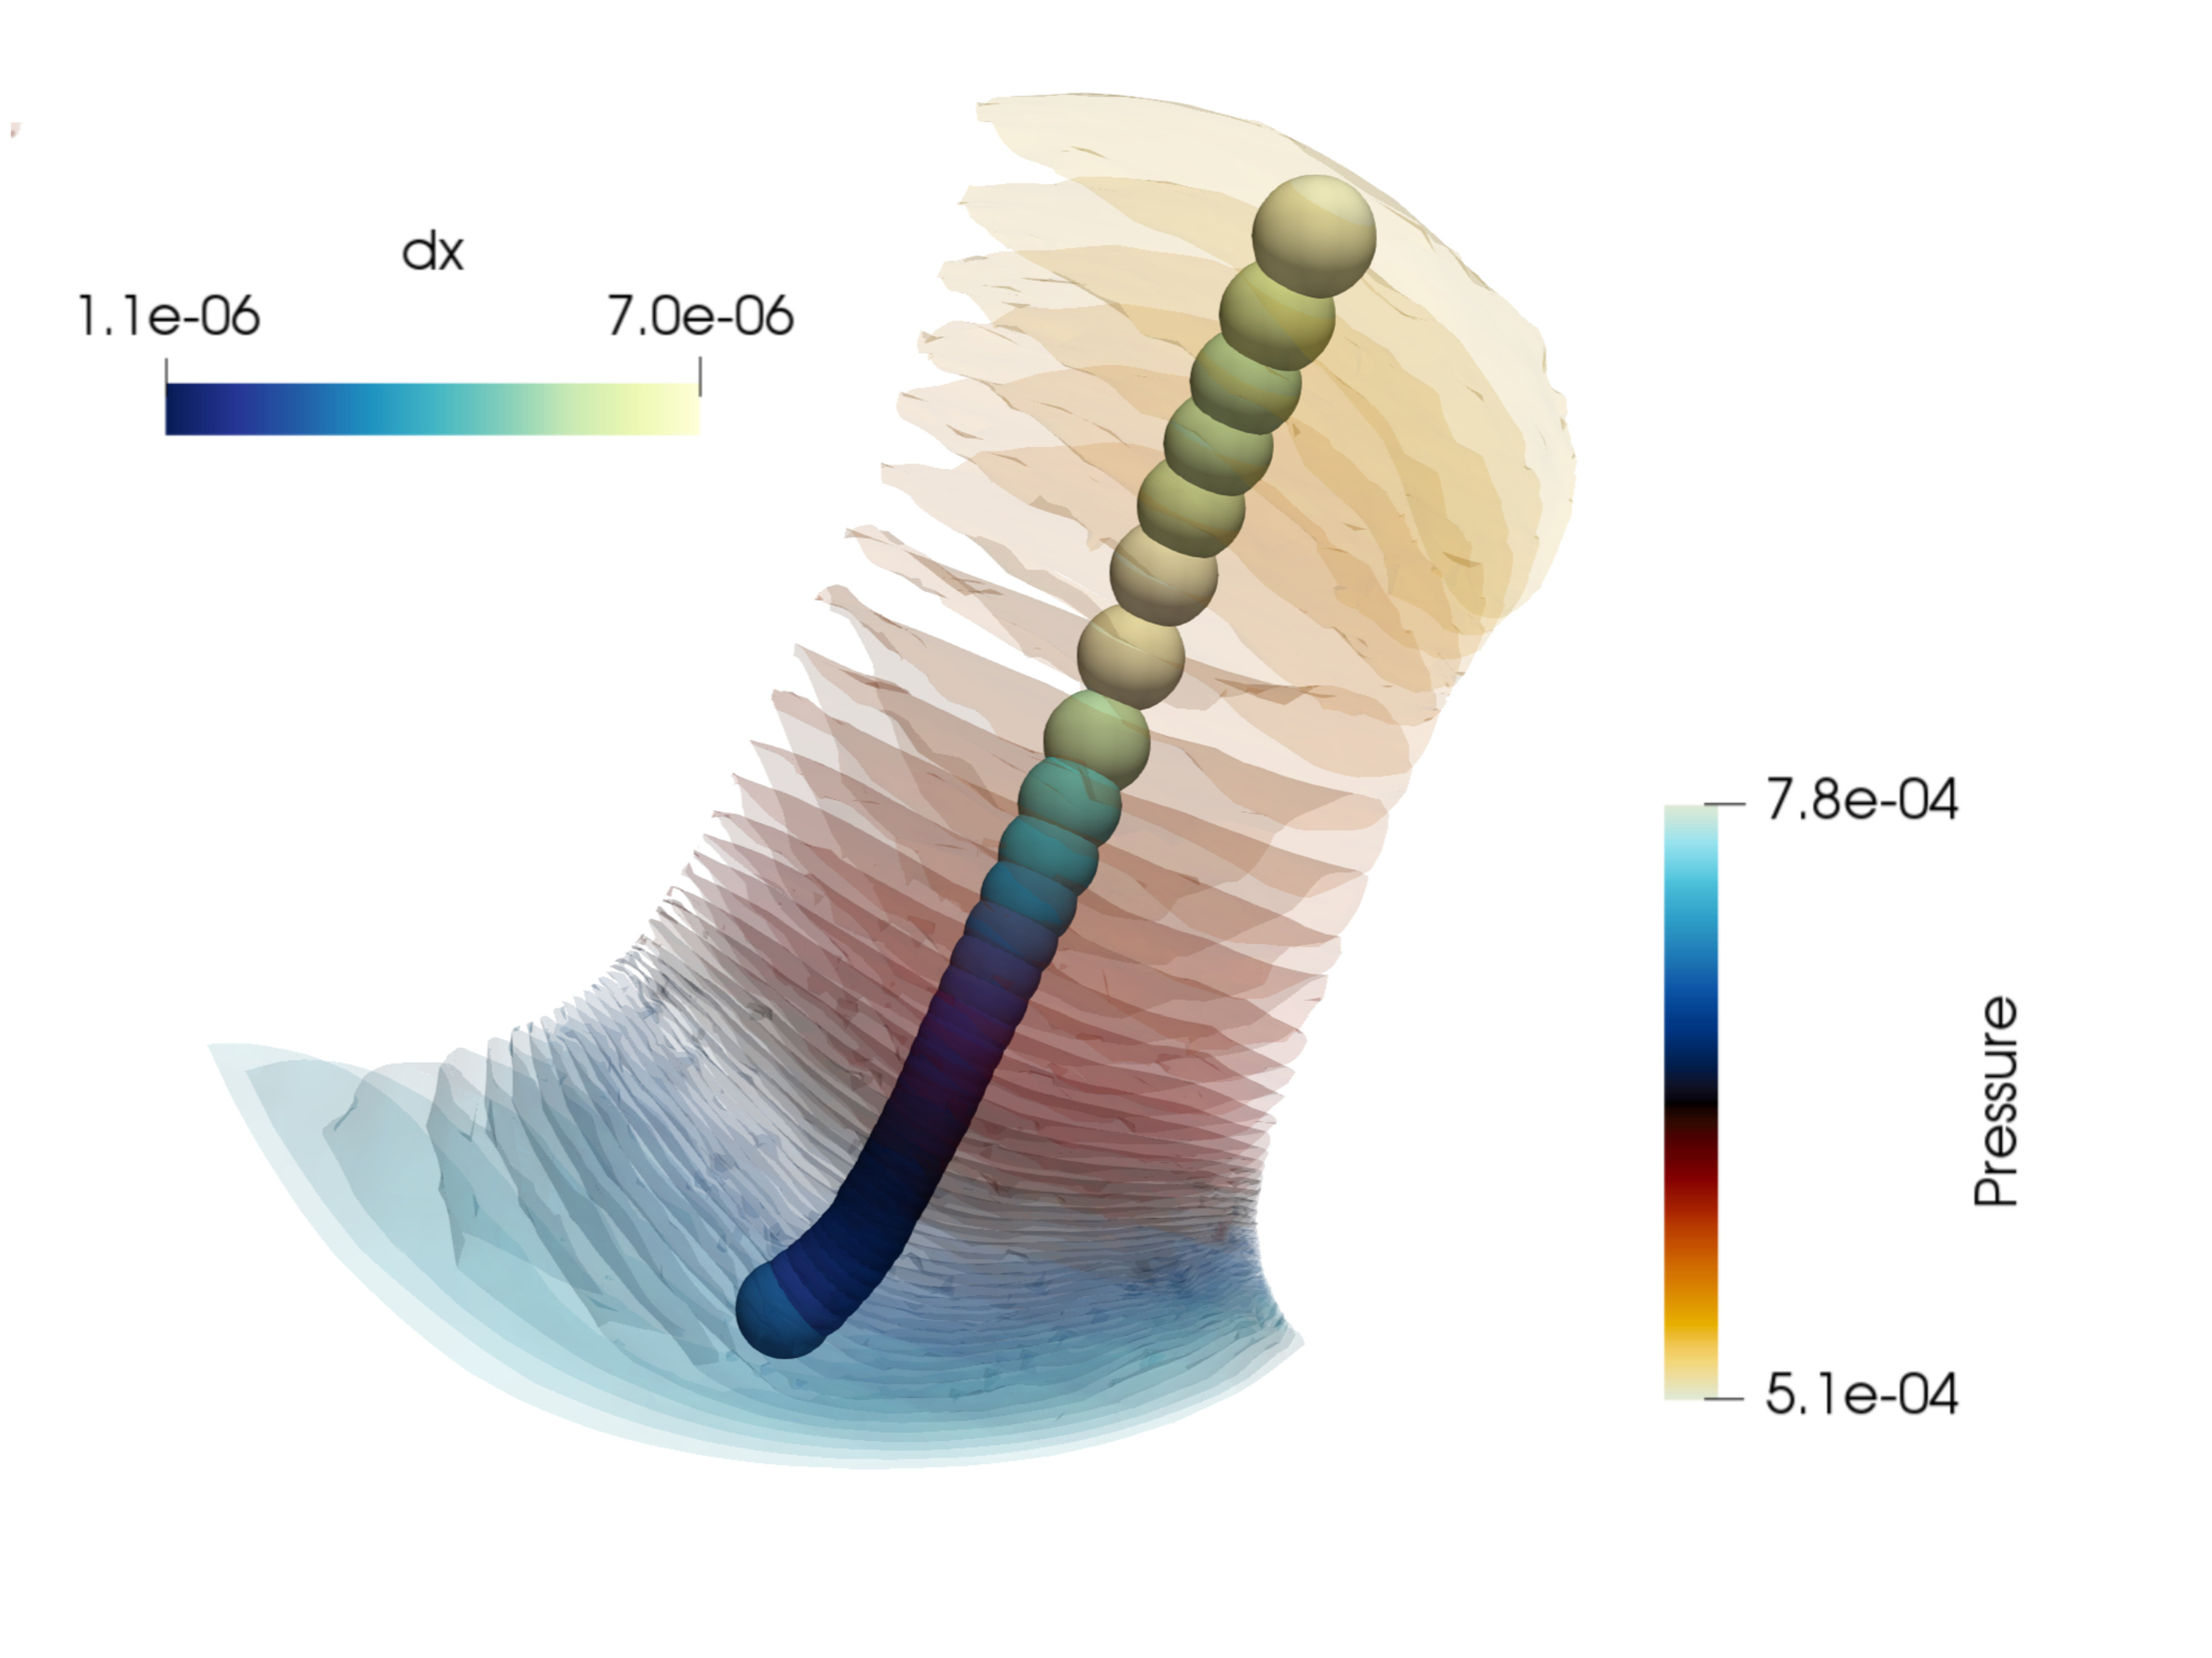
\includegraphics[height=5.5cm]{figures/example_pore_v2.eps}
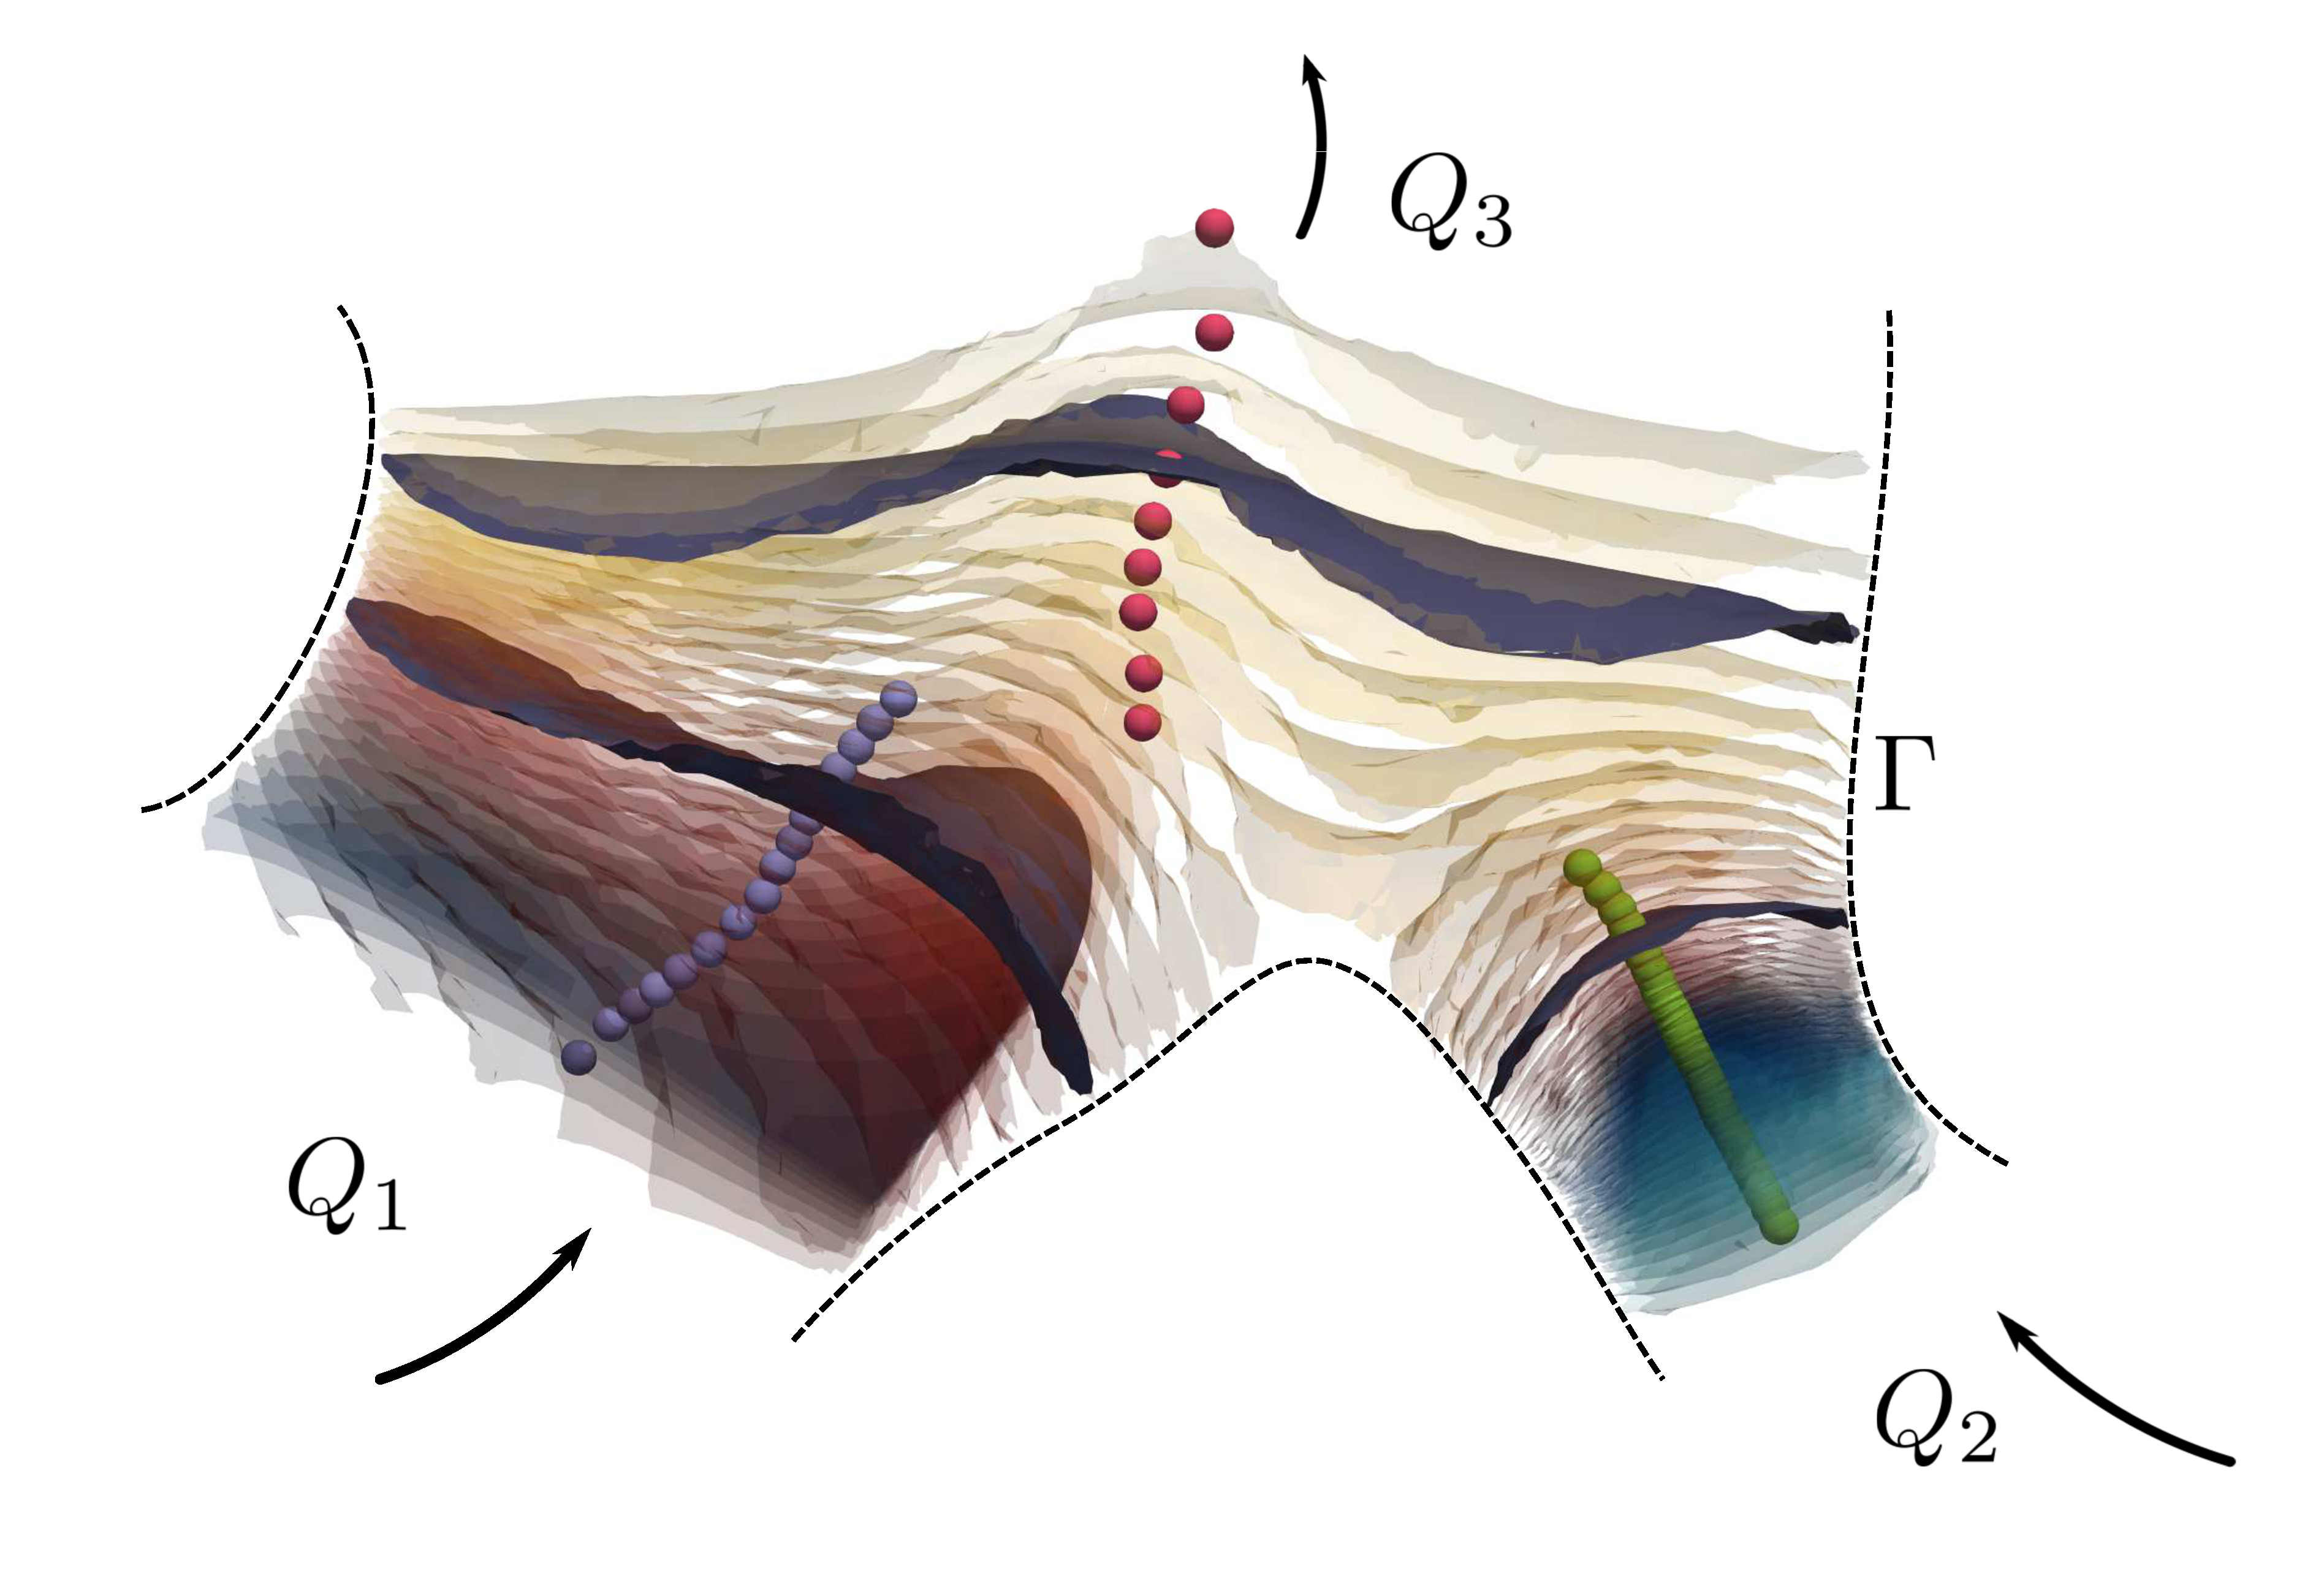
\includegraphics[height=5.5cm]{figures/merging_pores_v2.eps}
\caption{Left: A visualization of a collection of consecutive iso-pressure surfaces comprising one pore, including the center of mass of the iso-pressure surfaces indicated by the spheres. The color code of the spheres is given by the distance between the average coordinates between two consecutive iso-pressure surfaces. Right: A visualization of a junction of three pores for which the total flux is conserved $Q_1+Q_2 = Q_3$. This visualization is based on a subset of the DNS results of porous media \#2}
\label{fig:isop_surfaces}
\end{figure}
Here we introduce the notion of disconnected iso-pressure surface $\mathcal{S}_i(p)$ for a given pressure value $p$. Iso-pressure surfaces are usually disconnected because they exist in the fluid domain only and are thus interrupted by the solid phase of the media. The first term of Eq.~(\ref{eq:stokes_dissipation}), the boundary term, will be less significant when the total volume $V$ is enlarged by increasing $\delta p$. Furthermore, when we have saturated conditions, the complete pore space can be compartmentalized in a network of enclosed volumes $V_i(p_i, p_i+\delta p_i )$, which we will later call pores. For all the pore spaces in the network the boundary term only exists virtually, since the same boundary term is subtracted for the pores to which they are physically connected. Therefore Eq.~(\ref{eq:stokes_dissipation}) intrinsically only evaluates
\begin{equation}
Q \Delta p=\mu\int (\nabla \otimes \mathbf{u})^2 dV.\label{eq:pore_based_energy_dissipation}
\end{equation}

In the following we apply a decomposition of the velocity vector $\mathbf{u} = u_p \mathbf{\hat{p}} + u_r \mathbf{\hat{r}}$ with $\mathbf{\hat{p}} =\mathbf{ \nabla}p/|\mathbf{ \nabla}p|$ (longitudinal direction in respect to the flow) and $\hat{\mathbf{p}}$ perpendicular to $\hat{\mathbf{r}}$ (transversal direction in respect to the flow). We assume that the most important contributions to the viscous dissipation tensor $\nabla_i u_j$ are given by $\nabla_i u_p$ i.e. $\mathbf{\nabla}_i u_r \ll \mathbf{\nabla}_i u_p $. This assumption has been verified in the supplementary information (SI) for the porous media that we have used below and leads to 
\begin{equation}
\left|\nabla_i u_j\right|^2 \approx  \left|\nabla_r u_p\right|^2 + \left|\nabla_p u_p\right|^2 .\label{eq:reduced_dissipation_tensor}
\end{equation}
Here the first term is expected to be more important for gradually varying pore geometries since gradients in the velocity in the longitudinal direction are usually much lower than in transverse direction. Equations (\ref{eq:stokes_local})-(\ref{eq:reduced_dissipation_tensor}) are valid for arbitrary volumes $V$. When we consider viscous dissipation in an \textit{infinitesimal} volume $dV$ enclosed by $\mathcal{S}(p),\mathcal{S}(p+\delta p)$ (with respective areas $A(p), A(p+\delta p)$), separated by average distance $dx$ defined by $dV = A(p)dx$, we can estimate (analogous to \citeA{mortensen_reexamination_2005}) the average value of the first term of Eq.~(\ref{eq:reduced_dissipation_tensor}) by
\begin{equation}
	\left|\nabla_r u_p\right|^2 =8\pi \left(\alpha_0+\alpha_1\,\mathcal{C}\right)\frac{ Q^2}{A^3}~~~ ,\label{eq:tau_1}
\end{equation}
with circularity parameter $\mathcal{C} = \mathcal{L}^2/4\pi A(p)$ with perimeter $\mathcal{L} = \int_{\partial \mathcal{S}(p)}dl$. The circularity parameter is related to the compactness factor $C = \mathcal{C}/4\pi$ in \cite{mortensen_reexamination_2005}, and for HP flow it is equal to one. The coefficients $\alpha_0$ and $\alpha_1$ can be calculated (in first order of circularity) analytically or numerically for simple shapes of the iso-pressure surfaces, such as squares, triangles, or a perturbation of a sphere by spherical harmonics \cite{mortensen_reexamination_2005}. For heterogeneous media the class of shapes are generally unknown and not symmetric, and therefore $\alpha_0$ and $\alpha_1$ are expected to be intrinsically dependent on the pore geometry and therefore to change from pore to pore.  

For the second, longitudinal term, we can assume that the total flux $Q$ remains constant for $p\rightarrow p+dp$, and the change of the velocity in longitudinal direction is caused by a change in cross-sectional area $A(p)\rightarrow A(p+\delta p)$. We estimate $u_p$ by the total flux $Q/A$, i.e. 
\begin{equation}
	\left|\nabla_p u_p\right|^2 =  8\pi  \alpha_2\frac{Q^2}{A^4}\left|\frac{dA}{dx }\right|^2,\label{eq:tau_2}
\end{equation}
with proportionality factor $\alpha_2$. Again $\alpha_2$ is intrinsically dependent on pore geometry and changes from pore to pore. We combine the two expressions Eq.~(\ref{eq:tau_1}) and Eq.~(\ref{eq:tau_2}) with Eq.~(\ref{eq:pore_based_energy_dissipation}) into
\begin{equation}
	\frac{dp}{dx} = 8\pi \mu \frac{Q(p)}{A(p)^2} f\left(\alpha_i,\mathcal{S}(p) \right),\label{eq:infi_dp}
\end{equation}
with 
\begin{equation}
	 f\left(\alpha_i,\mathcal{S}(p)\right) = \alpha_0+\alpha_1\mathcal{C} + \alpha_2 \frac{1}{A}\left|\frac{d A}{d x}\right|^2.
\end{equation} 	
This parametrization is consistent with the Hagen-Poiseuille equation for pipe geometries $f(\alpha_i)\rightarrow 1$, for which the local infinitesimal pressure gradient is given by 
\begin{equation}
	\frac{d p}{d x} = 8 \pi \mu\frac{Q}{A^2}\label{eq:HP}.
\end{equation} 
As long as the total flux $Q$ remains constant and $dV = Adx$ remains valid, Eq.~(\ref{eq:infi_dp}) can be integrated over $\Delta p$. We define a pore by the integrated volume, bound by iso-pressure surfaces $\mathcal{S}_i(p)$, $\mathcal{S}_j(p+\Delta p)$ and the porous media boundary. The hydraulic resistance of a pore is then given by $\mathcal{R}= \frac{\Delta p}{Q}$. The right-hand side of Eq.~(\ref{eq:pore_based_energy_dissipation}) gives us therefore a statistical model for the hydraulic resistance $\mathcal{R}_m$ given by
\begin{equation}
	\mathcal{R}_m = \int^{L_{\rm{eff}}}_{0}\frac{1}{A^2}f\left(\alpha_i,\mathcal{S}(p)\right)\,dx\label{eq:R_model},
\end{equation}
with $L_{\rm{eff}}= \int\,dx $ the total effective length of the pore. When the geometry of a media is given by a long pipe, the hydraulic resistance is given by the Hagen-Poiseuille (HP) model $\mathcal{R}_{\rm{HP}}$, given by $\mathcal{R}_m(f\rightarrow 1)$. The HP model therefore only depends on the cross-sectional area $A(p)$.


\section{Methods}
\begin{figure}[t!]
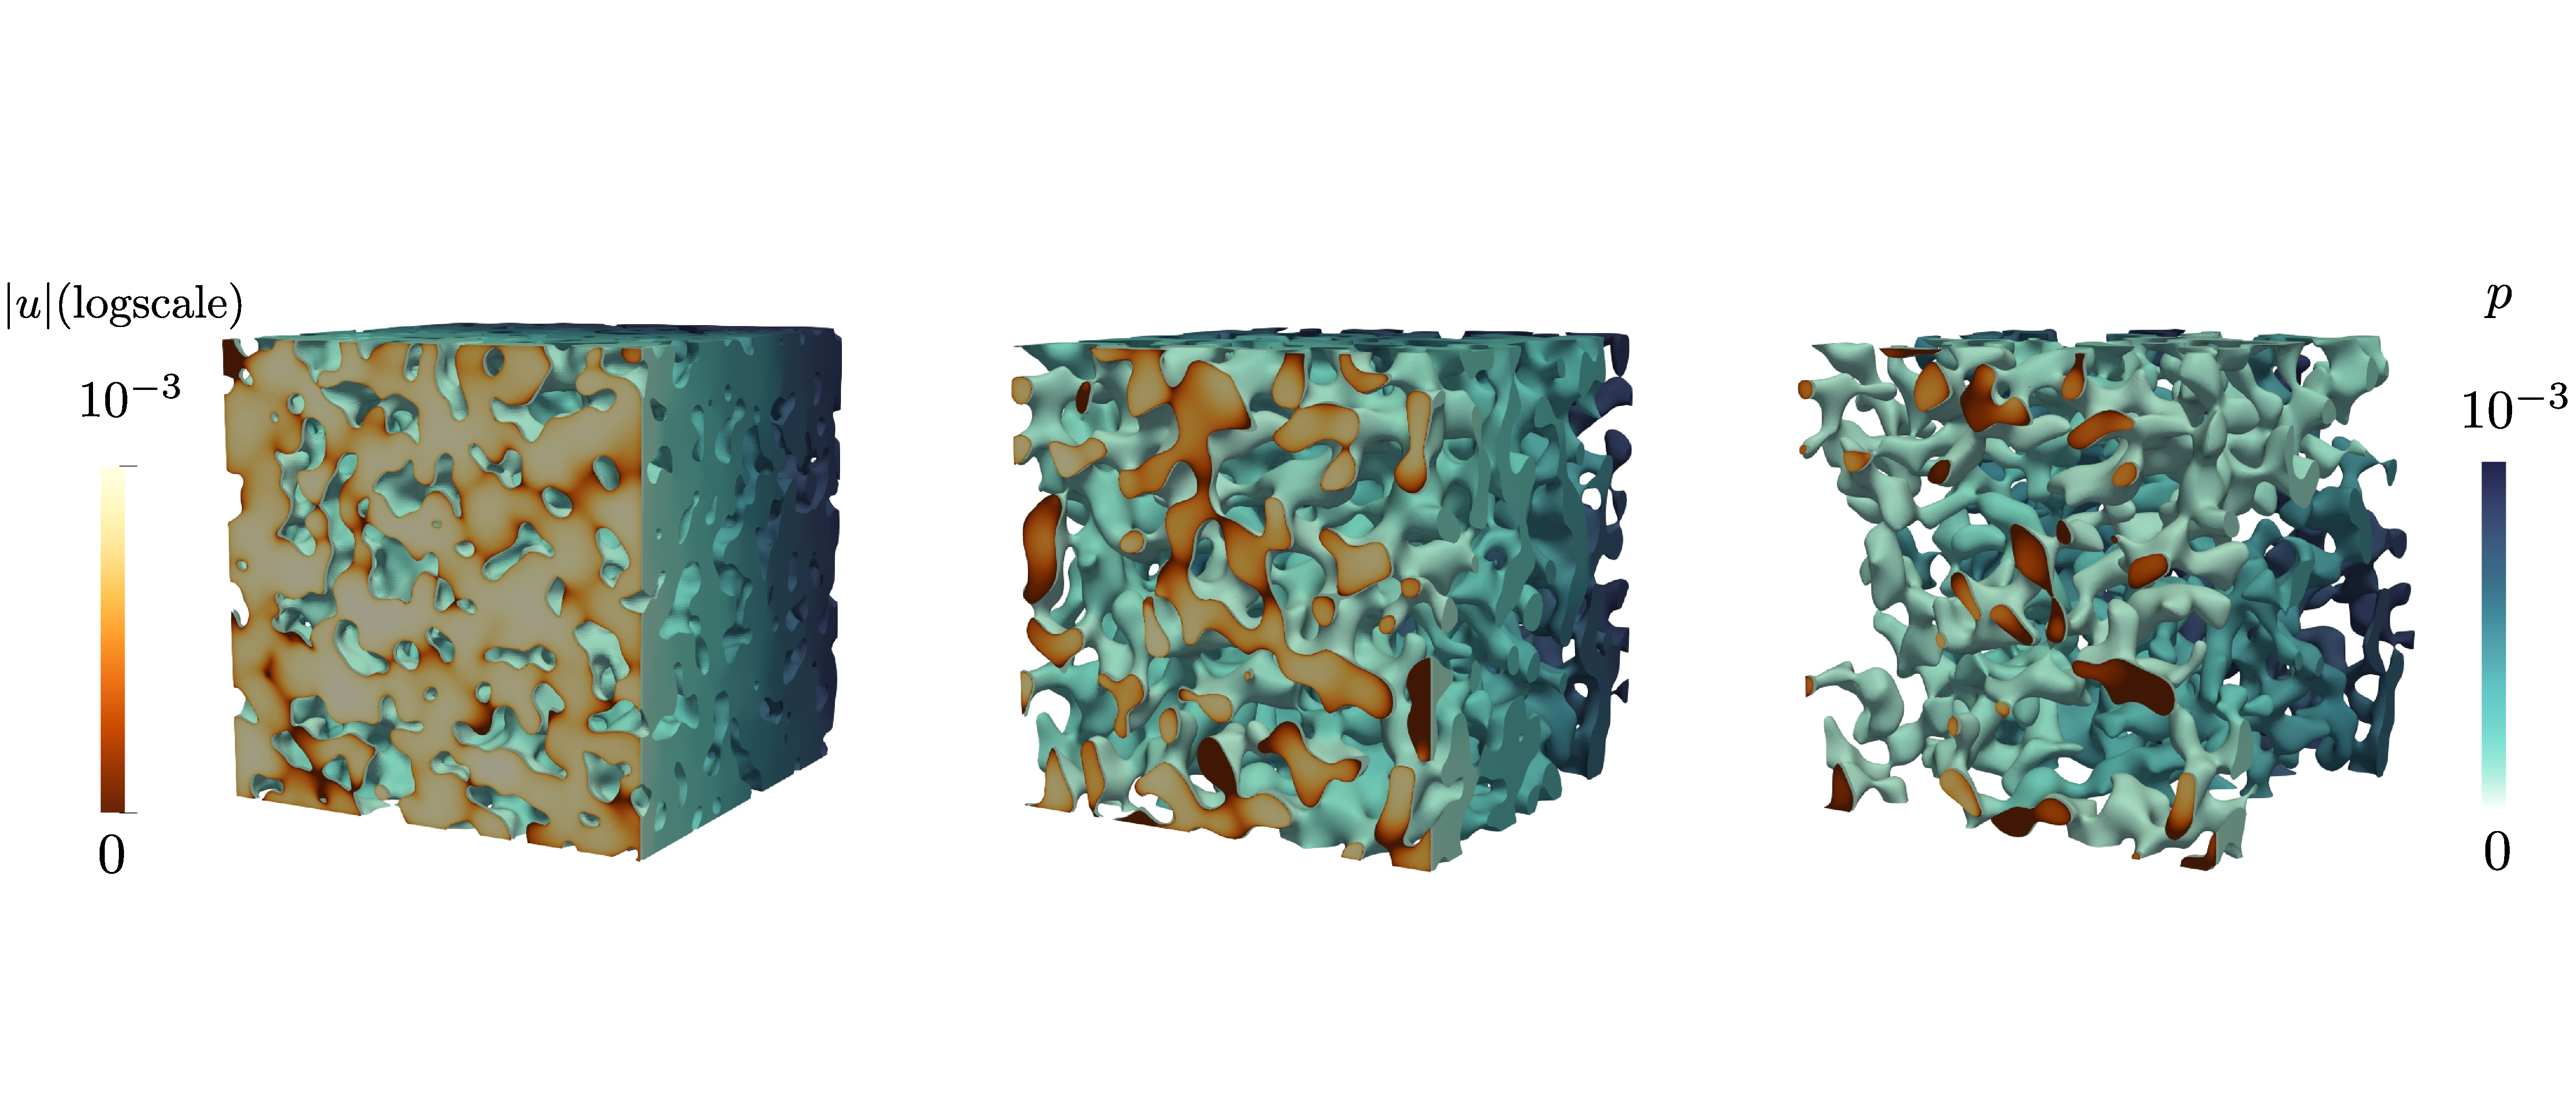
\includegraphics[width=1.0\linewidth]{figures/DNS_overview.eps}
\includegraphics[width=1.2\linewidth]{figures/infi_dpdx_3.pdf}
\caption{Top: A visualization of the velocity field $|u|$ and pressure field $p$ in the pore space of the three porous media used in this study. Bottom: Measurements of local pressure drop versus the Hagen-Poiseuille model given by Eq.~(\ref{eq:HP}) for three different porous media. The color is given by averaged circularity $\mathcal{C}(p)_i$ and the marker size is scaled with the averaged area $A(p)_i$ of two consecutive iso-pressure surfaces $\mathcal{S}(p)_i,\mathcal{S}(p+\delta p)_j$. }
\label{fig:DNS}
\end{figure}


To generate heterogeneous porous media we make use of the Gaussian Random Fields (GRF), which are increasingly used to represent realistic porous media \cite{liu_advances_2019}. We used a fast fourier transform and a spectral density function to generate GRF scalar functions \cite{teubner_level_1991,hyman_heterogeneities_2012,siena_relationship_2014}. A threshold on the GRF function is used to define the porous media-fluid interface $\Gamma$ with porosities $0.68, 0.34$ and $0.17$ respectively. For details on the GRF functions and geometrical parameters such as average pore size and surface roughness are given in the SI. These porous media are used as input for direct numerical simulations (DNS, OpenFOAM v. 4.1, \citeA{weller_tensorial_1998}), that solve the Stokes equations (Eq.~\ref{eq:stokes_local}) in the pore space. The boundary conditions are defined at the inlet $p_1$ and outlet $p_2$ and a no-slip condition for the porous media-fluid interface. A visualization of the three porous media is shown in Fig.~\ref{fig:DNS}. Next, a chain of visualization toolkit (VTK) based image analysis techniques \cite{schroeder_visualization_2006,hernderson_paraview_2007} is employed to extract iso-pressure surfaces $\mathcal{S}(p)$ and enumerate the disconnected areas identified as an iso-pressure patch $\mathcal{S}_i(p)$. This patch is part of a pore and has a surface area $A_i(p)$, circularity $\mathcal{C}_i(p)$, center of `mass' of iso-pressure surface $\mathbf{X}_i(p)$ and total flux $Q_i(p)$. For each $\mathcal{S}_i(p)$ we identify its closest neighbor $\mathcal{S}_j(p+\delta p)$. This neighboring iso-pressure patch (building up a pore) is found by calculating the distance function $f_d(\mathbf{x},\mathcal{S})$, between any given point $\mathbf{x}\in \mathcal{S}_i(p)$ and all iso-pressure patches $\mathcal{S}_k(p+\delta p)$. This distance function is defined by
\begin{equation}
	f_d\left(\mathbf{x},\mathcal{S}\right) = \min \{\Vert\mathbf{x}-\mathbf{y}\Vert \} ~|~ \mathbf{y}\in \mathcal{S}.
\end{equation}
for each $i,k$ we define the averaged distance matrix 
\begin{equation}
	d_{i,k} = \frac{1}{A_i(p)}\int_{\mathcal{S}_i(p)} f_d(\mathbf{x}_i,\mathcal{S}_k(p+\delta p)) \,dS_i.
\end{equation}
The closest neighbor $\mathcal{S}_j(p+\delta p)$ is found by the minimum value of $d_{i,j} = \rm{min}\left\{ d_{i,k}\right\}$. When $\delta p$ is chosen sufficiently small the enclosed volume can be estimated by $V_i(p,\delta p)=A_id x_i \approx A_i d_{i,j}$. We use forward integration of consecutive patches until merging or splitting takes place. This is translated into constraints on flux conservation and an upper bound for $d_{i,j}$. We noticed however that the distances between $\mathbf{X}_i(p)$ and $\mathbf{X}_j(p+\delta p)$ of two consecutive pores are more sensitive to topology changes, and are therefore used instead. The precise values for these constraints can be found in the SI. A demonstration of the correct identification of pores by forward integration is shown in Fig.~\ref{fig:isop_surfaces} (Right), showing a merging of two pores. Although the proposed definition of individual pores deals naturally with junctions, a straight forward pore-network implementation is still missing. This is partly due to the exclusion of iso-pressure patches that are singular, and have no neighboring patches due to rapid changing topologies. The percentages of excluded surface area patches are $18 \%,~26 \%$ and $2\%$, which, at least for the first two porous media, prevents a continuous reconstruction of the network-topology. This is not an issue for the present work which aims at validating the novel constitutive relation which is carried out for individual pores and a continuous pore network is not required. However, for a pore-network implementation of the approach to be applicable, this should be resolved in future work.

The main challenge with the data format of the OpenFoam simulations is that it is unstructured, and the meshing is refined towards the boundary of the porous media $\Gamma$. Although this ensures that the geometry is accurately described and that the simulation converges, it also causes challenges in the extraction of $\mathcal{S}(p)$ by using a VTK contour filter. Since it is based on a threshold on $p$ it breaks up the mesh close to $\Gamma$ into many disconnected noisy area patches. These are removed by applying a filter on the area size of the patches, resulting in a reduction of total surface area of maximally $1\%$. Extracting circularity $\mathcal{C}_i(p)$ is achieved by applying a contour filter on $\mathcal{S}_i(p)$ with a threshold on the velocity of $|u| = 0 $, obtaining the circumference $\mathcal{L}_i(p)$ of the area patch, practically infinitely close to the porous media boundary. The difference with respect to taking the contour exactly at the boundary introduces an averaged overestimation for $\mathcal{C}_i(p)$ by a factor $\epsilon = 1.15,~1.11,~1.08$ for the three porous media respectively. The origin of this error is the grid refinement near the boundary. Given that this is uniform throughout the porous media, we expect the error to be similar for all $\mathcal{C}_i(p)$. More information on this error estimate can be found in the SI. 

For each of the three porous media we evaluate Eq.~(\ref{eq:infi_dp}) for all consecutive iso-pressure pairs $\mathcal{S}_i(p)$. To obtain measured values for the resistance of a pore, we divide the total pressure difference $\Delta p$ by the total flux $Q$. We fit Eq.~(\ref{eq:R_model}), to all pores belonging to one porous media, yielding three sets of $\alpha_i$.  

\section{Results}


The result of the DNS for the three porous media is shown in Fig.~\ref{fig:DNS}. The Reynolds numbers are calculated by $\rm{Re} \sim \ell_p q/\nu$, with $q$ the average flux through the porous media and $\ell_p$ the average pore size defined by the total porous media volume to total porous media interface ratio $\ell_p = 4 \phi V/|\Gamma|$. For all porous media $\rm{Re}$ is smaller than $10^{-2}$. In Fig.~\ref{fig:DNS}, bottom, the results of the infinitesimal pressure gradients versus the HP model (Eq.~(\ref{eq:HP})) are shown. We observe that the HP model underestimates the pressure gradient by up to two orders of magnitude for the first porous media, to a relative good estimate for the third. We notice that $\mathcal{C}$ is the lowest for smallest pores, indicating that smaller iso-pressure surfaces are more circular than larger, more complex shaped iso-pressure surfaces. Besides the fact that the data covers different ranges we see no visual visual distinction between the three porous media, i.e. their data overlap and behave uniformly with respect to $\mathcal{C}$ and size $A$, see Fig.~\ref{fig:local_and_integrated}, top left.
 
For each porous media Eq.~(\ref{eq:infi_dp}) has been fitted by minimizing the least-squared error independently to obtain estimates for $\alpha_i$. The contribution of the term $\alpha_2$ is insignificant for all three porous media and is reported in the SI. A simple fit, excluding $\alpha_2$ resulted in three values for $\alpha_0 = 0.48, 0.52, 0.19$ and $\alpha_1 = 0.90, 0.87, 1.16$ for the corresponding porous media respectively. The result of the fitting is shown in Fig.~\ref{fig:local_and_integrated} (top, right). Using Eq.~(\ref{eq:infi_dp}) with the fitted values for $\alpha_0$ and $\alpha_1$ ($\alpha_2 = 0$) we obtain a new model for local pore resistances $\mathcal{R}_m$, Eq.~(\ref{eq:R_model}), which performs much better than the HP model. The result is shown in Fig.~\ref{fig:local_and_integrated} (bottom, right). We notice that obtained values for $\alpha_1$ are underestimated by $1/\epsilon$ given that the circularity is overestimated by $\epsilon$. 

The Pearson correlation coefficients $R^2$ for all models of the resistances are higher than $0.88$. For the HP model the values for $R^2$ are given by $0.91, 0.88$ and $0.99$. The coefficients $R^2$ of $\mathcal{R}_m$ are given by $0.97, 0.95$ and $0.99$. The high values are caused by the large domain size spanning several orders of magnitude. The deviations of $\mathcal{R}_{\rm{HP}}$ with the measured values $\Delta p/Q$ are not uniform across the scales and  therefore $R^2$ is not a reliable parameter when it comes to expressing the improvement over the HP model \cite{wilcox_comparing_2009}. We therefore calculated the reduction of the root-mean-squared-relative error (RMSRE) from $\mathcal{R}_{\rm{HP}}$ to $\mathcal{R}_{\rm{m}}$. For the first porous media we found a reduction in the RMSRE from $59\%$ to $12\%$, for the second from $46\%$ to $13\%$ and for the last from $31\%$ to $15\%$.  

\begin{figure}
\includegraphics[height=8cm]{figures/infi_dpdx_combined.pdf}
\includegraphics[height=8cm]{figures/integral_R_combined.pdf}
\caption{Top left: Measured infinitesimal pressure gradient versus the infinitesimal pressure drop of a Hagen-Poiseuille model, i.e. $f(\alpha)\rightarrow 1$, for all three porous media combined. The marker size is scaled with square root of the averaged area $\sqrt{\overline{A}}$. Top right: Measured versus Modeled infinitesimal pressure gradient with $f(\alpha)$ fitted to Eq.~(\ref{eq:infi_dp}) for each porous media separately. Bottom: The marker size is scaled by $N\sqrt{\overline{A}}$, with N the number of consecutive patches. Bottom left: Integrated pressure drop vs $\mathcal{R}_{HP}$ times the total Flux $Q$. Bottom right: Integrated pressure drop divided by the total Flux $Q$ vs $\mathcal{R}_m$ (Eq.~(\ref{eq:R_model})). }
\label{fig:local_and_integrated}
\end{figure}


Since we obtain a range of complex shapes for $\mathcal{S}$ the obtained values for $\alpha_i$ are expected to be an average.   Therefore it is interesting to test the robustness of the linearity in $\mathcal{C}$ and the consistency of the function $f \rightarrow 1$ when $\mathcal{C}\rightarrow 1$. We introduce an alternative function $g$ to $f$ with two fit parameters $\alpha$ and $\beta$,
\begin{equation}
	g(\mathcal{C}) = 1-\alpha\left[1-\left(\mathcal{C}/\epsilon\right)^{\beta}\right] \label{eq:R_model_uniform},
\end{equation}
with a reduction factor $1/\epsilon$ for $\mathcal{C}$ to compensate for the known overestimation of $\mathcal{C}$. This function is consistent with the HP model as long as $\beta =1$. The fitting resulted in three values for $\alpha = 0.45,~0.58,~0.34$, and $\beta = 1.09,~1.05,~1.08$. The latter suggesting that non-linear contributions of $\mathcal{C}$ can be present but are expected to be relatively small. A model including a quadratic term, reported in the SI, gives the same performance, but with the danger of over-fitting. By using $g(\mathcal{C})$ the RMSREs are higher than for the model resulting from fitting Eq.~(\ref{eq:R_model}). This is reflected in a central spread of $\mathcal{R}_m$ around the $1:1$ line, whilst with Eq.~(\ref{eq:R_model_uniform}), the model predicts generally values above the $1:1$ line. The Pearson correlation coefficients of the uniform model are similar, given by $R^2 = 0.97,~0.95$ and $0.99$ indicating a similar performance. All models and their parameters including performances are listed in the SI.
 

The range of local resistances in Fig.~\ref{fig:local_and_integrated} (bottom) show that low resistances are correlated with high values for $\mathcal{C}$, and are poorly estimated by the HP model. These pores are crucial for predicting preferential flow paths since they depend on the paths of least resistances throughout a network. For this purpose we have computed the RMSRE weighted by the mean flux. We found a reduction from $86\%, 60\%, 32\%$ for the HP model to $10\%, 12\%, 13\%$ for the new model for the three heterogeneous media respectively, which shows a remarkable improvement for high flux pores.  


\section{Discussion}

One of the most important findings is that the prediction of the resistance of a pore by $\mathcal{R}_{\rm{HP}}$ is highly underestimated with an average RMSRE of $0.45$. This is most pronounced when the pores have a complex geometry, which are usually correlated with large pore areas, see Fig.~\ref{fig:local_and_integrated}. An average underestimation of the resistances leads to an average overestimation of the mean fluxes in a network model. This will affect transport predictions e.g. breakthrough times will be underestimated \cite{dentz_mechanisms_2018}. Network models such as \cite{alim_local_2017}, often base their local resistances on the smallest distances to the porous media boundary. In general this will underestimate the cross-sections and therefore obtain higher resistances for the HP-based model, potentially reducing the error with respect to our HP model. Since anomalous diffusion has been correlated with the degree of heterogeneity of the porous media, it is important that low flux regions are included. The inaccurate representation of the low velocity regions of larger cross-sectional areas will therefore contribute to poor estimates of anomalously long residence times. Estimating these residence times properly is important because they underly non-Fickian scaling behavior of the dispersion of flow tracers \cite{dentz_mechanisms_2018,dentz_delay_2006}.

We expect that our main results are transferable to other media such as packed-beads, sandstone and disordered media, since iso-pressure surfaces are expected to be quite heterogeneous even if grains are regular. In ordered and/or high porosity media we expect iso-pressure surfaces that are highly connected, similar to porous media 1 in this paper, and sometimes even consisting of a singular patch. In these cases extracting statistics can be challenging. One possible strategy for separation of highly connected iso-pressure surfaces into smaller patches could be a watershed or Morse-Smale-Complex segmentation \cite{tierny_topology_2018}. 


One of the key observations of our work is the possibility of introducing a local geometric factor that provides for the ratio of pressure difference and mass flux in a given pore. The factor depends on the considered pore and not the rest of the complicated shape of the medium boundary. The non-triviality of this observation is made transparent by employing the boundary integral representation which is equivalent to the Stokes equations obeyed by the flow. The representation gives the flow as an integral over the medium surface where the points of the surface appear as sources that produce the flow as superposition. The ``charge" of such sources is proportional to the stress tensor at the boundary and the flow that each charge induces in space is given by an appropriate Green's function, see e.g. \cite{pozrikidis_boundary_1992}. Our result demonstrates that contributions other than those from the boundary of the considered pore can be neglected in the superposition. The mechanism by which this occurs, consists of both screening effect and destructive interference between different pores. This deserves further studies which are beyond our scope here. We have used circularity, as a single measure for the shape of $\mathcal{S}(p)_i$, but to improve on this result it might be necessary to include other shape parameters such as curvature measures of $\mathcal{S}(p)_i$, which however may lead to non-linear behavior in a circuit model. 

Although a pore-network implementation is still missing due to the incomplete evaluation of all surface area patches, an alternative option is to use a statistical network representation based on our results. Given that the distributions of the resistances show similarity with a log-normal distribution (see SI), a pathway for a statistical network based on these distributions seems feasible. 

\section{Conclusion}
We have proposed a new iso-pressure surface based definition for individual pores in heterogeneous porous media with the aim of measuring and modeling the local hydraulic resistance which can potentially be used in a pore-network model. This new definition uses the constant flux as constraint on the length of the pore. The definition of the pores allows us to estimate the local hydraulic resistance in terms of the viscous dissipation tensor. This can be modeled by Eq.~(\ref{eq:R_model}) containing the circularity of the iso-pressure surfaces. This model significantly improves the Hagen-Poiseuille model for heterogeneous media. 

\acknowledgments{The authors acknowledge support through SNSF grant nr.172916 and valuable discussions with H. L\"owe and V. L. Morales.}



\bibliography{library.bib}



\end{document}



